\documentclass[11pt]{article}
\usepackage[margin=1in]{geometry}
\usepackage[T1]{fontenc}
\usepackage{lmodern}
\usepackage{microtype}
\usepackage{amsmath,amssymb}
\usepackage{graphicx}
\usepackage{tikz}
\usetikzlibrary{arrows.meta,positioning}
\usepackage{array}
\usepackage{enumitem}
\usepackage[hidelinks]{hyperref}
\usepackage{url}
\urlstyle{sf}
% Figures compile with OR without the converted PDFs (convert paper/figures/*.svg).
\newcommand{\paperfig}[2]{\IfFileExists{#1}{\includegraphics[width=\linewidth]{#1}}%
{\fbox{\parbox{0.95\linewidth}{\centering\vspace{1.4em}\itshape #2\\[2pt]\textnormal{[figure placeholder --- convert the matching \texttt{figures/*.svg} to PDF]}\vspace{1.4em}}}}}
\title{OpenWOP as a Vendor-Neutral Workflow Orchestration Protocol}
\author{David S. Tufts\\
MyndHyve Inc.\\
\emph{\small OpenWOP project steward (see Positionality, Section~1)}\\
Grand Rapids, Michigan, USA\\
\url{https://davidtufts.me}\quad\url{https://www.linkedin.com/in/davidtufts}}
\date{June 2026}
\begin{document}
\maketitle

\begin{center}\small\itshape
Prepared by the OpenWOP project steward (see Positionality, Section 1); integrates reference-implementation, conformance, and cross-host portability evidence with appropriate scholarly caution.
\end{center}
\begin{abstract}
Multi-agent AI systems increasingly require durable, observable, interruptible, replayable, and portable workflow execution across heterogeneous hosts. This paper argues that a vendor-neutral open workflow orchestration protocol may be a necessary infrastructure layer for such systems. OpenWOP is examined as a candidate protocol because it standardizes the workflow run as the primary unit of orchestration, together with host capability discovery, run events, interrupts, artifacts, replay, observability, and conformance behavior. The paper is organized around three analytic dimensions: standardization, interoperability, and portability. It distinguishes OpenWOP from adjacent protocols: A2A supports inter-agent collaboration, while MCP supports tool, resource, prompt, and context integration. These protocols may compose in a full agentic architecture, but the paper's argument concerns the distinct need for open workflow orchestration. Implementation and conformance evidence strengthen the claim: the OpenWOP project includes a reference workflow-engine application and a public conformance leaderboard that records compatible hosts, advertised profiles, and scenario results. We further report a reproducible cross-language portability result: the same workflow definition executed across an independent TypeScript host and a Python host yields identical terminal state and event-log structure for core workflows. We treat these as evidence of implementability and internal consistency, not as proof of broad adoption or productivity gains. The contribution is a protocol-level argument and validation agenda for evaluating whether OpenWOP can reduce orchestration-layer fragmentation and support portable intelligent software workflows.
\end{abstract}
\section*{1. Introduction}
Agentic software systems are moving beyond isolated tool calls or single-agent sessions. They increasingly coordinate multiple agents, external tools, human approvals, policy checks, artifact generation, event streams, and long-running execution. This creates an orchestration-layer problem: teams need workflows that can be started, observed, interrupted, resumed, replayed, audited, and moved across systems without binding the workflow semantics to a single vendor or runtime.

The central thesis of this paper is that a vendor-neutral open protocol for multi-agent workflow orchestration can accelerate intelligent software development by standardizing workflow communication, reducing integration complexity, and enabling portability across tools, systems, and organizational boundaries. This should be read as a scholarly argument and research hypothesis, not as a fully established empirical claim. The paper therefore distinguishes protocol-level claims from adoption and productivity claims that require further study.

OpenWOP is a useful case because its specification corpus frames it as an open protocol for portable, durable, AI-native workflow execution across hosts [1]. Independent surveys of the agent-protocol landscape distinguish tool/context integration (MCP) and agent-to-agent collaboration (A2A) from durable workflow control [31, 32]; OpenWOP occupies the last of these. It does not replace A2A or MCP; it fills the orchestration-layer gap that remains when multi-step agentic work must be durable, observable, replayable, and portable.

Positionality. This manuscript is authored by the steward of the OpenWOP project, not by an independent third party. All reference hosts, the conformance suite, and the demo application analyzed here are steward-produced; the conformance leaderboard is self-reported. No independent, non-steward host or maintainer exists at the time of writing. We therefore treat implementation and conformance material as evidence of implementability and internal consistency, never as third-party validation or adoption, and we flag throughout where a claim would require an independent party to establish. This stance is a deliberate threat-to-validity control, stated up front so the evidence below is read correctly.

\section*{2. Problem: Orchestration-Layer Fragmentation}
The current agentic ecosystem includes many useful frameworks, runtimes, and integration protocols. However, their abstractions are often framework-specific, runtime-specific, or vendor-specific. Coordination logic is frequently embedded in proprietary orchestration surfaces, custom adapters, or one-off workflow state models. This creates three forms of fragmentation:

\begin{itemize}[leftmargin=*]
\item Semantic fragmentation: systems represent tasks, runs, interrupts, artifacts, approvals, and lifecycle states differently.
\item Integration fragmentation: workflow clients, hosts, agents, tools, and observability systems require bespoke adapters.
\item Portability fragmentation: workflow definitions, event histories, artifacts, and replay/debug data often cannot move cleanly across hosts.
\end{itemize}
The problem is not the absence of workflow engines or agent frameworks. The problem is the absence of a shared, vendor-neutral wire contract for durable AI workflow execution. A workflow engine can execute work; an orchestration protocol specifies how clients and hosts interoperate across organizational and implementation boundaries.

\section*{3. Contribution}
This paper makes three contributions:

\begin{enumerate}[leftmargin=*]
\item It defines orchestration-layer fragmentation as a distinct research problem in agentic software systems.
\item It analyzes OpenWOP as a vendor-neutral workflow orchestration protocol organized around standardization, interoperability, and portability.
\item It proposes a validation agenda for evaluating cross-host execution, event-log fidelity, human-checkpoint semantics, replay, conformance, and integration-complexity reduction.
\end{enumerate}
\section*{4. Related Work}
OpenWOP sits at the intersection of four bodies of work. The contribution is not a new execution engine but a vendor-neutral wire contract for the orchestration layer; related work is organized by what OpenWOP deliberately does not duplicate.

Durable-execution runtimes. Temporal, Cadence, Restate, DBOS, AWS Step Functions, and Azure Durable Functions provide durable, replayable, long-running execution [6, 8, 9]. They solve execution, the problem an OpenWOP host solves internally, but each exposes a proprietary, runtime-specific surface that cannot move across runtimes. OpenWOP instead standardizes the client-host boundary so durable execution becomes portable across independently-implemented hosts, of which a Temporal-class engine could be one: the distinction is a database engine versus the SQL wire protocol.

Vendor-neutral workflow standards, and why portability did not follow. OpenWOP is not the first attempt at a portable workflow standard. WS-BPEL, XPDL, BPMN, and more recently CNCF Serverless Workflow and Argo Workflows aimed at portable, declarative definitions [12, 15, 16] (see also [13, 14]). The lesson is directly relevant: a portable definition format did not yield portable execution, because those standards specified the static graph but left lifecycle, event semantics, human checkpoints, replay, and capability negotiation to each engine. OpenWOP's wager is that portability lives in the runtime contract, not the definition language, which is why its kernel centers the Run, the EventLog, Interrupt/ResumePayload, and a ConformanceProfile rather than only a WorkflowDefinition.

Agent protocols. The Model Context Protocol standardizes an application's access to tools, resources, prompts, and context [17]; Agent2Agent standardizes inter-agent discovery and delegation [18]; agent-framework orchestration such as LangGraph, AutoGen, and CrewAI embeds coordination inside a single runtime [19, 20, 21]. OpenWOP occupies the layer none of these own: durable, observable, replayable, portable workflow control across hosts.

LLM-native workflow orchestration, and the protocol proliferation. A distinct and very recent line of work treats workflow orchestration itself as an LLM capability: DSPy's declarative, self-improving LM pipelines [26], AFlow's automated workflow-graph search [28], and WorkflowLLM, which fine-tunes orchestration ability and frames the shift from Robotic Process Automation to Agentic Process Automation [27]; the space is mapped by recent surveys from static templates to dynamic runtime graphs [34]. In parallel, a wave of agent-communication protocols (MCP, A2A, ACP, ANP) has appeared and is catalogued by dedicated protocol surveys [31, 32] and broad multi-agent surveys [29, 30]. These are complementary to OpenWOP and sharpen its gap rather than fill it: workflow-generation systems optimize the workflow graph but assume a runtime to execute it; agent protocols standardize how agents discover and message one another, not how a multi-step run is durably executed, observed, interrupted, replayed, and certified across hosts. The proliferation of competing agent protocols is itself evidence of the orchestration-layer fragmentation this paper names. The emerging agent-reliability literature, such as Byzantine-fault-tolerance perspectives on multi-agent systems [33], further motivates the durable-execution and replay guarantees OpenWOP elevates into a portable, conformance-tested contract.

Two further recent threads reinforce this positioning. First, record-and-replay and determinism are being brought directly to LLM agents - logging only non-deterministic events to reconstruct state [35], building deterministic LLM workflows [36], and characterizing why even temperature-zero inference drifts [37] - which is exactly why OpenWOP records non-determinism as pins in the event log rather than regenerating it at fork time. Second, the agent-evaluation literature is itself fragmenting [38], and a unified evaluation framework recently showed that scaffold and framework choice materially shift agent outcomes [39] - direct external evidence that agent behavior is not portable across implementations today, the gap a conformance-tested wire contract is meant to close.

Observability, replay, and event sourcing. OpenWOP's EventLog and replay/fork model applies event sourcing and deterministic replay [22, 23], and its TraceContext aligns with OpenTelemetry's propagation model [24]. The novelty is not the mechanism but its elevation into a cross-vendor protocol obligation with conformance scenarios, so the guarantee is portable rather than per-runtime.

Standardization as the mechanism. The thesis that a vendor-neutral protocol accelerates an ecosystem has precedent worth citing as analogy rather than proof: TCP/IP, SQL, HTTP, and OpenTelemetry each decoupled an interoperability layer from competing implementations and enlarged the market [25, 40, 24]. We invoke these as motivating analogy and mark the acceleration claim as a long-term hypothesis.

Positioning summary. Against durable-execution runtimes, OpenWOP is the wire contract they could share; against prior workflow standards, it standardizes the runtime contract they omitted; against MCP and A2A, it is the complementary orchestration layer; against event-sourcing practice, it makes those guarantees a portable protocol obligation. No prior artifact offers a vendor-neutral, conformance-tested, run-centered orchestration contract spanning lifecycle, human checkpoints, replay, and capability discovery.

\section*{5. OpenWOP Protocol Kernel}
Rather than restate the entire v1 specification corpus, we focus on a minimal protocol kernel. The core abstraction is the Run: a durable execution instance that can be created, observed, interrupted, resumed, completed, failed, cancelled, replayed, or forked.

\begin{table}[h]\centering\footnotesize
\begin{tabular}{>{\raggedright\arraybackslash}p{0.307\textwidth}>{\raggedright\arraybackslash}p{0.307\textwidth}>{\raggedright\arraybackslash}p{0.307\textwidth}}\hline
\textbf{Kernel construct} & \textbf{Protocol role} & \textbf{Paper relevance} \\\hline
Run & Primary unit of durable workflow execution & Replaces vague workflow language with a concrete unit of standardization \\\hline
HostCapabilityDocument & Discovery surface for supported protocol features, limits, profiles, and transports & Enables clients to reason about host behavior before execution \\\hline
WorkflowDefinition & Portable description of executable work & Supports workflow reuse and cross-host portability \\\hline
RunEvent / EventLog & Ordered record of lifecycle and execution events & Supports observability, audit, replay, and evidence \\\hline
Interrupt / ResumePayload & Human or external control point and continuation payload & Makes HITL checkpoints first-class workflow semantics \\\hline
Artifact & Structured result or intermediate output & Preserves outputs across runs, hosts, and integrations \\\hline
TraceContext & Correlation identifiers for observability systems & Links protocol events to production monitoring \\\hline
ConformanceProfile & Declared behavior plus scenario evidence & Provides testable portability and compatibility claims \\\hline
\end{tabular}\end{table}
Why these constructs, and why this few. The kernel is not an arbitrary selection from the v1 corpus; it is the minimal set of obligations the client-host boundary must fix for a workflow to move across independently-implemented hosts. Each construct corresponds to a distinct interoperability failure that arises if the obligation is left to the host, the failure mode that defeated definition-only standards such as BPMN:

\begin{itemize}[leftmargin=*]
\item HostCapabilityDocument prevents blind, non-negotiable integration: without machine-readable discovery, capability mismatches surface only at runtime.
\item WorkflowDefinition is necessary but, as BPMN and Serverless Workflow show, not sufficient on its own.
\item Run and RunEvent/EventLog locate portability where it actually lives, the execution record: two hosts interoperate only if the same definition yields the same observable event sequence. This is the construct prior standards omitted.
\item Interrupt/ResumePayload makes human and external checkpoints first-class rather than a per-vendor extension.
\item Artifact prevents result lock-in across runs, hosts, and integrations.
\item TraceContext prevents per-runtime observability silos.
\item ConformanceProfile turns every claim above into a testable, evidence-backed assertion.
\end{itemize}
Removing any one construct reintroduces a vendor-specific surface at that seam; adding agent cognition or tool protocols would exceed the boundary and duplicate MCP and A2A. The kernel is thus the fixed point adjacent systems only partially provide: durable-execution runtimes have a Run and an event history but no portable discovery, definition, or conformance contract; workflow standards have a definition but no event-log, interrupt, or conformance semantics; MCP and A2A have neither a Run nor an EventLog. OpenWOP's contribution is precisely the union none of them expose as a shared, conformance-tested contract, and that union is what cross-host portability requires.

\begin{figure}[h]\centering
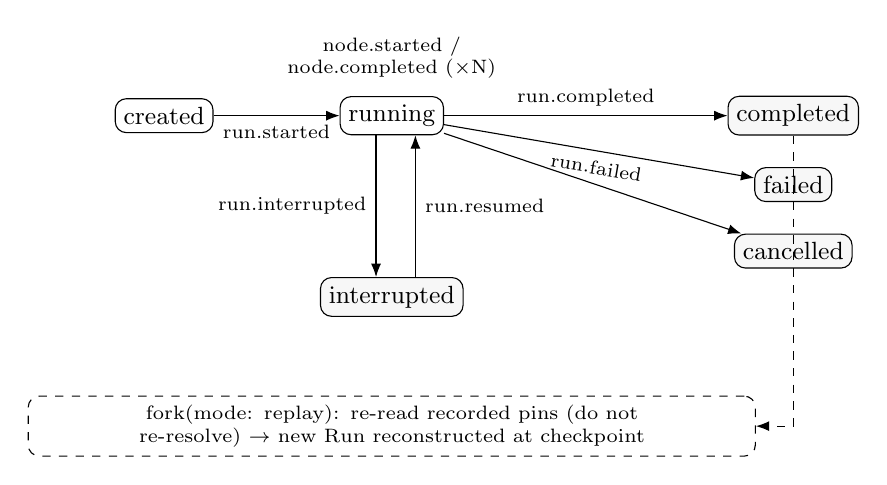
\begin{tikzpicture}[every node/.style={font=\small},>=Latex,node distance=16mm]
\node[draw,rounded corners,inner sep=3pt] (cr) {created};
\node[draw,rounded corners,inner sep=3pt,right=of cr] (run) {running};
\node[draw,rounded corners,fill=black!3,inner sep=3pt,right=36mm of run] (done) {completed};
\node[draw,rounded corners,fill=black!3,inner sep=3pt,below=4mm of done] (fail) {failed};
\node[draw,rounded corners,fill=black!3,inner sep=3pt,below=4mm of fail] (canc) {cancelled};
\node[draw,rounded corners,fill=black!3,inner sep=3pt,below=18mm of run] (intr) {interrupted};
\node[font=\scriptsize,above=1mm of run,align=center] {node.started /\\ node.completed ($\times$N)};
\draw[->] (cr) -- node[below,font=\scriptsize]{run.started} (run);
\draw[->] (run) -- node[above,font=\scriptsize]{run.completed} (done);
\draw[->] (run) -- node[sloped,below,font=\scriptsize]{run.failed} (fail);
\draw[->] (run) -- (canc);
\draw[->,transform canvas={xshift=-2mm}] (run) -- node[left,font=\scriptsize]{run.interrupted} (intr);
\draw[->,transform canvas={xshift=3mm}] (intr) -- node[right,font=\scriptsize]{run.resumed} (run);
\node[draw,dashed,rounded corners,align=center,font=\scriptsize,below=10mm of intr,text width=9cm] (fork)
 {fork(mode: replay): re-read recorded pins (do not re-resolve) $\to$ new Run reconstructed at checkpoint};
\draw[->,dashed] (done.south) |- (fork.east);
\end{tikzpicture}
\caption{Run lifecycle state machine. States are observable as RunEvents on the append-only EventLog; terminal states are completed, failed, or cancelled; interrupt/resume make human checkpoints first-class; fork replays from a recorded checkpoint into a new Run. The node-execution sequence shown was captured identically on the TypeScript and Python reference hosts.}
\end{figure}
\section*{6. Secondary Scope Boundaries: A2A and MCP}
A2A and MCP are secondary here; they matter because they prevent overclaiming. A2A addresses independent agents discovering and delegating work to one another. MCP addresses model, tool, resource, prompt, and context integration. OpenWOP addresses durable workflow orchestration. Recent protocol surveys catalogue this layered landscape and treat the three as complementary rather than substitutes [31, 32].

\begin{figure}[h]\centering
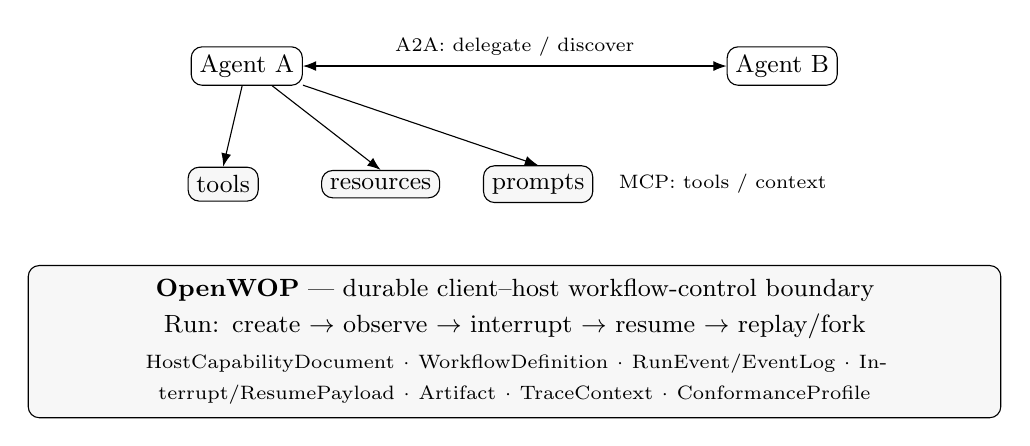
\begin{tikzpicture}[every node/.style={font=\small},>=Latex]
\node[draw,rounded corners,inner sep=3pt] (a) at (0,3.2) {Agent A};
\node[draw,rounded corners,inner sep=3pt] (b) at (6.8,3.2) {Agent B};
\draw[<->] (a) -- node[above,font=\scriptsize]{A2A: delegate / discover} (b);
\node[draw,rounded corners,fill=black!3,inner sep=3pt] (t1) at (-0.3,1.7) {tools};
\node[draw,rounded corners,fill=black!3,inner sep=3pt] (t2) at (1.7,1.7) {resources};
\node[draw,rounded corners,fill=black!3,inner sep=3pt] (t3) at (3.7,1.7) {prompts};
\draw[->] (a) -- (t1.north); \draw[->] (a) -- (t2.north); \draw[->] (a) -- (t3.north);
\node[font=\scriptsize,anchor=west] at (4.6,1.7) {MCP: tools / context};
\node[draw,rounded corners,fill=black!3,align=center,text width=12cm,inner sep=5pt] at (3.4,-0.3)
 {\textbf{OpenWOP} --- durable client--host workflow-control boundary\\[2pt]
  Run: create $\to$ observe $\to$ interrupt $\to$ resume $\to$ replay/fork\\[2pt]
  {\scriptsize HostCapabilityDocument $\cdot$ WorkflowDefinition $\cdot$ RunEvent/EventLog $\cdot$ Interrupt/ResumePayload $\cdot$ Artifact $\cdot$ TraceContext $\cdot$ ConformanceProfile}};
\end{tikzpicture}
\caption{The three agent-era protocols are complementary, not substitutes. MCP standardizes an agent's vertical access to tools, resources, prompts, and context; A2A standardizes horizontal agent-to-agent delegation; OpenWOP standardizes the durable client-host workflow-control boundary that wraps a multi-step Run.}
\end{figure}
\begin{table}[h]\centering\footnotesize
\begin{tabular}{>{\raggedright\arraybackslash}p{0.307\textwidth}>{\raggedright\arraybackslash}p{0.307\textwidth}>{\raggedright\arraybackslash}p{0.307\textwidth}}\hline
\textbf{Question} & \textbf{Best protocol boundary} & \textbf{Why this matters for the paper} \\\hline
Should one agent ask another agent to do work? & A2A & This is collaboration, not workflow orchestration. \\\hline
Should an AI app or workflow node access tools, data, prompts, or context? & MCP & This is capability access, not durable workflow control. \\\hline
Should a multi-step workflow be started, streamed, interrupted, resumed, replayed, and validated? & OpenWOP & This is the orchestration-layer problem addressed by the paper. \\\hline
\end{tabular}\end{table}
\section*{7. Evidence Posture: Reference Implementation and Conformance}
The evidence basis is now stronger than a purely conceptual proposal. The project provides a hosted workflow-engine reference/demo application and an open repository for it. We treat this as reference-implementation evidence --- that the protocol can be represented in a working application and used to demonstrate run-oriented workflow behavior --- not as proof of broad adoption or production maturity.

The public conformance page is more directly usable as standards evidence. It describes a live record of OpenWOP-compatible hosts, their advertised compatibility profiles, and conformance scenario results. It also states that a host's place in the matrix is both a claim and evidence: the claim is the advertised profile, and the evidence is the conformance result published with the host or in the repository [2].

\begin{table}[h]\centering\footnotesize
\begin{tabular}{>{\raggedright\arraybackslash}p{0.307\textwidth}>{\raggedright\arraybackslash}p{0.307\textwidth}>{\raggedright\arraybackslash}p{0.307\textwidth}}\hline
\textbf{Evidence source} & \textbf{Supports} & \textbf{Does not yet prove} \\\hline
OpenWOP v1 spec corpus & Protocol scope and wire-contract intent & Adoption or implementation quality \\\hline
workflow-engine reference/demo app & Implementability and practical representation of the protocol & Cross-host portability or production deployment maturity \\\hline
Conformance leaderboard & Host compatibility claims, profiles, and scenario evidence & Universal conformance, ecosystem-wide adoption, or long-term stability \\\hline
A2A/MCP/OpenWOP comparison document [3] & Scope boundaries and complementary architecture & Need for OpenWOP by itself \\\hline
\end{tabular}\end{table}
\section*{8. Standardization, Interoperability, and Portability}
\subsection*{8.1 Standardization}
OpenWOP standardizes the boundary between workflow clients and workflow hosts. The standardization target is not agent cognition, model internals, tool protocols, or vendor runtime implementation. It is the durable workflow contract: run creation, lifecycle events, human checkpoints, artifacts, replay/debug surfaces, observability hooks, capability discovery, and conformance expectations.

\subsection*{8.2 Interoperability}
The interoperability claim is that workflow clients and hosts can communicate through shared run-level semantics rather than bespoke integrations. A client should be able to determine what a host supports, start a workflow, subscribe to events, respond to interrupts, retrieve artifacts, and understand terminal state without depending on a proprietary runtime model.

\subsection*{8.3 Portability}
Portability is the most demanding claim and the one we test directly. We operationalize it as follows: OpenWOP is portable for a workflow W if executing the same WorkflowDefinition against two independently-implemented compliant hosts yields, after normalizing host-local non-determinism, the same terminal RunState and the same canonical ordered sequence of RunEvent types.

We ran this across two reference hosts that are independent implementations in different languages, a TypeScript in-memory host and a stdlib-only Python host, driving identical conformance workflows through POST /v1/runs and reading each run's event log. For all three executable core workflows tested (conformance-noop, conformance-delay, and the multi-node conformance-multi-node), both hosts reached the identical terminal state (completed) and emitted the identical canonical event-type sequence. The multi-node case yielded, on both hosts:

\begin{center}\small\texttt{run.started -> node.started -> node.completed -> node.started -> node.completed -> node.started -> node.completed -> run.completed}\end{center}
The raw events differed exactly where the contract does not bind (event-identifier scheme, empty-payload representation, an optional sequence field) and matched exactly where it does (event-type order and terminal state). That two independent-language implementations agree on the contract while disagreeing on these incidental choices is the portability signal.

The experiment also surfaced a real divergence. The conformance-identity workflow references a node type (core.identity) that neither host advertises; both correctly declined to execute it, so the outcome is portable, but the failure mechanics differed: the Python host rejected the run at creation (HTTP 422, capability\_required) while the TypeScript host accepted it and failed the node (run.failed). The specification does not yet fix when a host must reject a workflow referencing an unadvertised node type; this is a concrete, portability-relevant tightening opportunity that our method detected.

Two limits bound this result. First, both hosts are steward-authored: this establishes cross-language consistency, not third-party independence. Second, the workflows are small and exercise only core execution; portability of interrupt/resume, replay/fork, and artifact-bearing workflows remains to be demonstrated across durable hosts. Full portability across genuinely independent hosts therefore remains a hypothesis, but it now rests on a reproducible result rather than assertion.

\begin{figure}[h]\centering
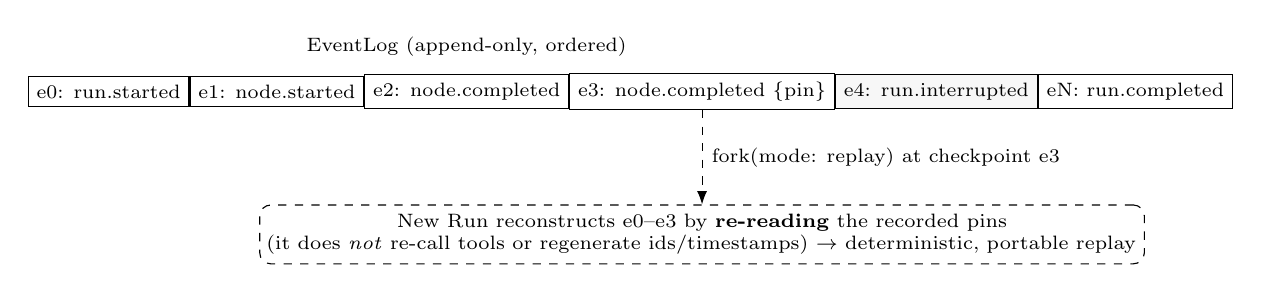
\begin{tikzpicture}[every node/.style={font=\scriptsize},>=Latex]
\node[draw,inner sep=3pt] (e0) {e0: run.started};
\node[draw,inner sep=3pt,right=0mm of e0] (e1) {e1: node.started};
\node[draw,inner sep=3pt,right=0mm of e1] (e2) {e2: node.completed};
\node[draw,inner sep=3pt,right=0mm of e2] (e3) {e3: node.completed \{pin\}};
\node[draw,inner sep=3pt,fill=black!3,right=0mm of e3] (e4) {e4: run.interrupted};
\node[draw,inner sep=3pt,right=0mm of e4] (eN) {eN: run.completed};
\node[font=\scriptsize,above=1mm of e2] {EventLog (append-only, ordered)};
\node[draw,dashed,rounded corners,align=center,below=12mm of e3,text width=11cm] (rc)
 {New Run reconstructs e0--e3 by \textbf{re-reading} the recorded pins\\(it does \emph{not} re-call tools or regenerate ids/timestamps) $\to$ deterministic, portable replay};
\draw[->,dashed] (e3.south) -- node[right,font=\scriptsize]{fork(mode: replay) at checkpoint e3} (rc.north);
\end{tikzpicture}
\caption{The append-only EventLog is the Run's source of truth; non-deterministic inputs are recorded as pins, and fork(mode: replay) reconstructs state by re-reading those pins rather than re-resolving them, which is what makes replay deterministic and portable.}
\end{figure}
\section*{9. Validation Agenda}
We frame validation as a ladder from minimum to stronger evidence per target. As of this version we have reached the stronger rung for implementability (a runnable reference host), event-log fidelity (schema-validated logs), interrupt/resume (an automated suspend--resume capture on a durable host), and portability for core workflows (the same definition on two independent-language hosts); the open rungs are an independent, non-steward host and a measured integration-complexity comparison.

\begin{table}[h]\centering\footnotesize
\begin{tabular}{>{\raggedright\arraybackslash}p{0.307\textwidth}>{\raggedright\arraybackslash}p{0.307\textwidth}>{\raggedright\arraybackslash}p{0.307\textwidth}}\hline
\textbf{Validation target} & \textbf{Minimum evidence} & \textbf{Stronger evidence (status this version)} \\\hline
Implementability & Reference workflow-engine demo shows run-oriented UI and protocol concepts & Runnable reference host with published commands and fixtures --- \emph{reached} \\\hline
Event-log fidelity & Sample observed run events and terminal state & Replayable event log with schema validation --- \emph{reached} \\\hline
Interrupt/resume semantics & Screenshot or transcript of pause/resume flow & Automated suspend--resume capture on a durable host (incl. the 422 negative path) --- \emph{reached} \\\hline
Conformance & Public leaderboard row and scenario results (reached) & Independent host passing core profile scenarios --- \emph{open} \\\hline
Portability & Host capability comparison & Same workflow on two language hosts; terminal state + event sequence equivalent (artifacts untested) --- \emph{reached for core} \\\hline
Integration reduction & Qualitative adapter mapping & Before/after code or adapter-count comparison --- \emph{open} \\\hline
\end{tabular}\end{table}
\section*{10. Claims and Evidence Discipline}
\begin{table}[h]\centering\footnotesize
\begin{tabular}{>{\raggedright\arraybackslash}p{0.307\textwidth}>{\raggedright\arraybackslash}p{0.307\textwidth}>{\raggedright\arraybackslash}p{0.307\textwidth}}\hline
\textbf{Claim} & \textbf{Current treatment} & \textbf{Required next evidence} \\\hline
OpenWOP defines a durable workflow orchestration protocol & Spec-supported claim & Continue citing spec corpus and kernel constructs \\\hline
OpenWOP complements A2A and MCP & Scope-supported claim & Keep secondary; cite the independent protocol surveys [31, 32] \\\hline
OpenWOP is implementable in practice & Reference-implementation- and run-capture-supported: captured HostCapabilityDocument, conformance snapshot, and reference- plus durable-host run logs & Independent (non-steward) deployment; production maturity \\\hline
OpenWOP conformance can be evaluated & Conformance-snapshot-supported: host rows, profiles, suite version, and pass rates captured & An independent host passing the core profile \\\hline
OpenWOP improves portability & Demonstrated for core workflows across two language hosts; durable-host interrupt/resume captured (Cell A) & Cross-host durable comparison (a second durable host) and an independent non-steward host \\\hline
OpenWOP reduces integration complexity & Hypothesis & Adapter count, code size, or integration-effort comparison \\\hline
OpenWOP accelerates intelligent software development & Long-term research claim & Empirical study or case evidence \\\hline
\end{tabular}\end{table}
\section*{11. Limitations and Threats to Validity}
We make the limitations explicit. First, a reference implementation and demo app establish implementability but not broad adoption. Second, conformance rows establish profile claims and scenario evidence, but not universal compatibility. Third, portability is not proven until the same workflow can be executed across independent hosts with preserved semantics. Fourth, productivity acceleration is a plausible downstream hypothesis, not a demonstrated result. Fifth, protocol standardization may be premature if the kernel is too broad; we therefore emphasize a minimal core plus profiles and extensions.

Construct validity. Our portability result operationalizes 'portable' as equivalence of terminal RunState and canonical RunEvent type-sequence after normalizing host-local non-determinism. This captures observable-contract equivalence, but it is narrower than full portability: it does not establish semantic equivalence of arbitrary workflows, equivalence of artifact contents beyond the cases tested, performance or operational portability, or developer-experience portability. Two hosts could agree on the measured sequence while differing in untested behavior. We therefore scope the portability claim to the constructs the tested workflows exercise, and treat the measure as a deliberate, falsifiable proxy rather than a complete definition. Because both hosts are steward-authored (see Positionality, Section 1), the result speaks to cross-language consistency of one author's implementations, not to reproducibility by an independent party.

\section*{12. Conclusion}
A vendor-neutral workflow orchestration protocol is a plausible infrastructure mechanism for reducing fragmentation in agentic software systems. OpenWOP should be evaluated as a protocol for durable workflow runs, not as a replacement for agent-to-agent collaboration, tool/context integration, or workflow runtimes. Its strongest scholarly contribution is the combination of a run-centered protocol kernel, observable event logs, human checkpoint semantics, replay/debug support, host capability discovery, and conformance evidence. This manuscript converts the earlier conceptual argument into an artifact-backed submission: demo and interrupt transcripts, a conformance snapshot, and a cross-host portability experiment accompany it. The decisive next evidence is a non-steward host and independent external review.

\section*{13. Reproducibility and Artifact Status}
The items that earlier drafts listed as immediate next steps have been carried out; the accompanying evidence artifact records the results, so they are reported here as status rather than as pending work.

\begin{table}[h]\centering\footnotesize
\begin{tabular}{>{\raggedright\arraybackslash}p{0.46\textwidth}>{\raggedright\arraybackslash}p{0.46\textwidth}}\hline
\textbf{Item} & \textbf{Status} \\\hline
Demo / run-lifecycle evidence & Done --- a reference-host run-event log, the live HostCapabilityDocument, and (on a durable host) the full interrupt/resume lifecycle (suspend $\to$ signed-token, correlation-validated external resume $\to$ \texttt{run.completed}, including the HTTP~422 mismatch path) plus the replay/debug bundle are captured. Deterministic fork-from-checkpoint replay remains future work. \\\hline
Conformance snapshot & Done --- leaderboard host rows, advertised profiles, suite version, and pass rates. \\\hline
Workflow-engine setup path & Done --- reference-host run commands, repository paths, and known limitations documented in the artifact. \\\hline
Artifact package + README & Done --- reviewer-facing README plus the evidence tree. \\\hline
References normalized & Done --- 40-entry bibliography, each entry verified against its authoritative source. \\\hline
Cross-host portability & Done (core) --- the same workflow definition yields identical terminal state and event-log structure across an independent TypeScript host and a Python host (3/3 core workflows), plus a capability-rejection divergence finding. \\\hline
External review & Reviewer packet prepared; feedback pending (the one step that requires external participants). \\\hline
Venue package & Done --- this arXiv-ready source (compiles to a 12-page PDF), the Word manuscript, an artifact archive, a cover note, and arXiv submission metadata. A shorter workshop-length version is left to a specific workshop venue's template, as arXiv imposes no page limit. \\\hline
\end{tabular}\end{table}
\begin{thebibliography}{99}
\raggedright  % ragged-right reference entries: no interword stretching -> no underfull-hbox warnings
\bibitem[1]{ref1} OpenWOP v1 specification corpus. \url{https://openwop.dev/spec/v1/}.
\bibitem[2]{ref2} OpenWOP Conformance leaderboard. \url{https://openwop.dev/conformance/}.
\bibitem[3]{ref3} OpenWOP --- A2A vs MCP vs OpenWOP. Project comparison document (steward-authored, not peer-reviewed), June 2026.
\bibitem[4]{ref4} OpenWOP reference hosts (in-memory, SQLite, Python, Postgres). \url{https://github.com/openwop/openwop-examples/tree/main/examples/hosts}.
\bibitem[5]{ref5} Hosted OpenWOP reference UI: \url{https://app.openwop.dev/}.
\bibitem[6]{ref6} Temporal. Documentation. \url{https://docs.temporal.io/}.
\bibitem[7]{ref7} Cadence (Uber). \url{https://cadenceworkflow.io/}.
\bibitem[8]{ref8} Restate. \url{https://restate.dev/}.
\bibitem[9]{ref9} A. Skiadopoulos, Q. Li, P. Kraft, K. Kaffes, et al. DBOS: a DBMS-oriented operating system. PVLDB 15(1):21-30, 2021.
\bibitem[10]{ref10} AWS Step Functions. Documentation. \url{https://docs.aws.amazon.com/step-functions/}.
\bibitem[11]{ref11} Azure Durable Functions. Documentation. \url{https://learn.microsoft.com/azure/azure-functions/durable/}.
\bibitem[12]{ref12} OMG. Business Process Model and Notation (BPMN) v2.0. formal/2011-01-03. \url{https://www.omg.org/spec/BPMN/2.0/}.
\bibitem[13]{ref13} OASIS. Web Services Business Process Execution Language (WS-BPEL) v2.0. 2007.
\bibitem[14]{ref14} WfMC. XML Process Definition Language (XPDL) 2.2. 2012. \url{https://wfmc.org/}.
\bibitem[15]{ref15} CNCF Serverless Workflow specification. \url{https://serverlessworkflow.io/}.
\bibitem[16]{ref16} Argo Workflows. \url{https://argo-workflows.readthedocs.io/}.
\bibitem[17]{ref17} Model Context Protocol (MCP) specification. \url{https://modelcontextprotocol.io/}.
\bibitem[18]{ref18} Agent2Agent (A2A) Protocol Specification. Linux Foundation, 2025. \url{https://a2a-protocol.org/latest/specification/}.
\bibitem[19]{ref19} LangGraph. \url{https://langchain-ai.github.io/langgraph/}.
\bibitem[20]{ref20} Microsoft AutoGen. \url{https://microsoft.github.io/autogen/}.
\bibitem[21]{ref21} CrewAI. \url{https://docs.crewai.com/}.
\bibitem[22]{ref22} M. Fowler. Event Sourcing. 2005. \url{https://martinfowler.com/eaaDev/EventSourcing.html}.
\bibitem[23]{ref23} R. O'Callahan, C. Jones, N. Froyd, K. Huey, A. Noll, N. Partush. Engineering Record and Replay for Deployability. USENIX ATC 2017.
\bibitem[24]{ref24} OpenTelemetry specification. \url{https://opentelemetry.io/docs/specs/}.
\bibitem[25]{ref25} M. L. Katz, C. Shapiro. Network Externalities, Competition, and Compatibility. American Economic Review 75(3):424-440, 1985.
\bibitem[26]{ref26} O. Khattab, A. Singhvi, et al. DSPy: Compiling Declarative Language Model Calls into Self-Improving Pipelines. arXiv:2310.03714, 2023 (ICLR 2024).
\bibitem[27]{ref27} S. Fan et al. WorkflowLLM: Enhancing Workflow Orchestration Capability of Large Language Models. arXiv:2411.05451, 2024.
\bibitem[28]{ref28} J. Zhang et al. AFlow: Automating Agentic Workflow Generation. arXiv:2410.10762, ICLR 2025.
\bibitem[29]{ref29} A Survey on LLM-based Multi-Agent Systems: Recent Advances and New Frontiers in Application. arXiv:2412.17481, 2024.
\bibitem[30]{ref30} Multi-Agent Collaboration Mechanisms: A Survey of LLMs. arXiv:2501.06322, 2025.
\bibitem[31]{ref31} A Survey of AI Agent Protocols. arXiv:2504.16736, 2025.
\bibitem[32]{ref32} A. Ehtesham et al. A Survey of Agent Interoperability Protocols: MCP, ACP, A2A, and ANP. arXiv:2505.02279, 2025.
\bibitem[33]{ref33} Rethinking the Reliability of Multi-agent Systems: A Perspective from Byzantine Fault Tolerance. arXiv:2511.10400, 2025.
\bibitem[34]{ref34} L. Yue et al. From Static Templates to Dynamic Runtime Graphs: A Survey of Workflow Optimization for LLM Agents. arXiv:2603.22386, 2026.
\bibitem[35]{ref35} E. Feng et al. Get Experience from Practice: LLM Agents with Record \& Replay. arXiv:2505.17716, 2025.
\bibitem[36]{ref36} L. Qiu et al. Blueprint First, Model Second: A Framework for Deterministic LLM Workflow. arXiv:2508.02721, 2025.
\bibitem[37]{ref37} Understanding and Mitigating Numerical Sources of Nondeterminism in LLM Inference. arXiv:2506.09501, 2025.
\bibitem[38]{ref38} A Survey on Evaluation of LLM-based Agents. arXiv:2503.16416, 2025.
\bibitem[39]{ref39} P. Zhu et al. A Unified Framework for the Evaluation of LLM Agentic Capabilities. arXiv:2605.27898, 2026.
\bibitem[40]{ref40} C. Shapiro, H. R. Varian. Information Rules: A Strategic Guide to the Network Economy. Harvard Business School Press, 1999.
\end{thebibliography}
\end{document}
